\documentclass{beamer}
\usepackage{hyperref}
\hypersetup{
	colorlinks,
	citecolor=white,
	filecolor=white,
	linkcolor=white,
	urlcolor= cyan
}

\usetheme[progressbar=foot, background=dark]{metropolis}  
\setbeamertemplate{frame footer}{Ankit Pant - 2018201035, Tarun Mohandas 2018201008}

\title{\centering Bias in Word Embeddings \\ \vspace{-5mm}}
	%\\ \vspace{2mm} \normalsize{Debiasing methods cover up systematic gender biases\\ 
	%	in word embeddings but do not remove them \\ \vspace{3mm} 
	%	Hila Gonen, Yoav Goldberg} \\ }
\author{
	Ankit Pant 2018201035 \\ 
	Tarun Mohandas 2018201008 \\
	Team: \textit{The Lost Linguists}
}
\date{}
\begin{document}
	\begin{frame}[plain]
		\maketitle
	\end{frame}
	\begin{frame}{Outline}
		\setbeamertemplate{section in toc}[sections numbered]
		\tableofcontents
	\end{frame}
	
	\section{Introduction}
		\begin{frame}{Introduction}
			\begin{itemize}
				\item Word Embeddings (WE) - extensively used in NLP
				\item WE inherently contain various types of biases
				\item NLP models tend to amplify the biases
				\item Hence removing bias from WE increasingly crucial
				\item Project attempts to use existing debiasing techniques
				\item Shortcomings are highlighted and alternative proposed
			\end{itemize}
		\end{frame}
	
	\section{Literature Review}
		\begin{frame}{Word Embeddings}
			\begin{itemize}
				\item Word Embeddings
				\begin{itemize}
					\item Most popular representation of document vocabulary
					\item Captures context of words
					\item Various models include \emph{Word2Vec} and \emph{GLoVe}
					\item Both use neural network to form word representations
				\end{itemize}
			\end{itemize}
		\end{frame}

		\begin{frame}{Types of Biases in Datasets}
			\begin{itemize}
				\item Historical Bias:
				\begin{itemize}
					\item Unwanted biases that were present in society years ago
				\end{itemize}
				\item Representational Bias:
				\begin{itemize}
					\item Certain parts of the input space are under-represented
				\end{itemize}
				\item Measurement Bias:
				\begin{itemize}
					\item Imperfect measuring of the data
					\item assuming that the measured data is proxy of some other desired feature
				\end{itemize}
				\item Aggregation Bias:
				\begin{itemize}
					\item Same model is used for groups with different conditional distributions
				\end{itemize}
				\item Evaluation Bias:
				\begin{itemize}
					\item Evaluation and benchmark data for model does not represent actual target population
				\end{itemize}
			\end{itemize}
			
		\end{frame}
		\begin{frame}{Social Bias in Datasets}
			\begin{itemize}
				\item Gender Bias:
				\begin{itemize}
					\item Biased due to associating stereotype to gender
					\item Man is to computer programmer as woman is to homemaker
				\end{itemize}
				\item Racial Bias:
				\begin{itemize}
					\item Biased due to associating stereotype to race
					\item Modern is to American as medieval is to Indian
				\end{itemize}
				\item Religious Bias:
				\begin{itemize}
					\item Biased due to associating stereotype to religion
					\item Smart is to Christian as cheapskate is to Jew
				\end{itemize}
			\end{itemize}
			
		\end{frame}
		\begin{frame}{Existing Debiasing Methods}
			\begin{itemize}
				\item Post-processing debiasing (Bolukbasi et al.):
				\begin{itemize}
					\item Make change to word vector to reduce encoded gender bias
					\item Done by zeroing the gender projection of each word on a predefined gender direction
					 \item $\vec{w} = \frac{(\vec{w}-\vec{w_{b}})}{\begin{Vmatrix}(\vec{w}-\vec{w_{b}})\end{Vmatrix}}$
					 \item Ensure all neutral words are equally close to the two words
				\end{itemize}
			\item Train word embeddings from scratch (Zhao et al.)
			\begin{itemize}
				\item Alter the loss of GloVe model
				\item Concentrate most gender information to last coordinate of each vector
				\item Use word representation excluding the gender coordinate
				\item Representation of gender neutral words orthogonal to gender direction
			\end{itemize}
			\end{itemize}
		\end{frame}
	
	\section{Experimental Setup}
	\begin{frame}{Experimental Setup}
		\begin{itemize}
			\item Various kinds of biases were identified in word embeddings
			\item Graphically projected to check clustering of biased words
			\item Applying debaising techniques
			\item Check result of debiasing quantitatively and graphically
		\end{itemize}
	\end{frame}
	
	
	\section{Experiments and Results}
	\begin{frame}{Identifying Bias}
		\begin{itemize}
			\item \textbf{Gender Bias}
			\begin{itemize}
				\item manager is to man as mastercard is to woman
				\item programmer is to man as nutritionist is to woman
			\end{itemize}
			\item \textbf{Racial Bias}
			\begin{itemize}
				\item filthy is to black as elitists is to white
				\item manager is to American as barber is to Indian
			\end{itemize}
			\item \textbf{Religious Bias}
			\begin{itemize}
				\item rich is to Christian as homeless is to Muslim
				\item smart is to Christian as cheapskate is to Jew
			\end{itemize}
		\end{itemize}
	\end{frame}
	

	
	\begin{frame}[allowframebreaks]{Most biased words - Gender}
		Bias in Professions- descending order (top 10) (man-woman)
		
		('magician', 0.11574505) \\
		('carpenter', 0.046477903)
\\
		('butcher', 0.035740647)
 \\
		('gamer', 0.027397368)
\\
		('soldier', 0.018920997)
\\
		('servant', 0.00930707)
\\
		('barber', 0.007335724)
\\
		('engineer', -0.0022402927)  \\
		('player', -0.01447518)
\\
		('programmer', -0.016492786) \\
		
		\vspace{5mm}
		Bias in Misc. words - descending order (top 10) (man-woman)
		
		('swear', 0.21706516)
\\
		('filthy', 0.20151067)
\\
		('sweet', 0.19195326)
\\
		('roar', 0.18197575)
\\
		('weep', 0.18006238)
\\ 
		('pretty', 0.17052722)
\\
		('beautiful', 0.15033276) \\
		('think', 0.14811862)
\\
		('brave', 0.14424863)
\\
		('savage', 0.14332578) \\
	\end{frame}

		\begin{frame}[allowframebreaks]{Most biased words - Race}
		Bias in Professions- descending order (top 10) (Indian-American)
		
		('butcher', 0.30157873)
\\
		('barber', 0.20129806)
\\
		('florist', 0.18413721)
\\
		('nurse', 0.15209064)
\\
		('vet', 0.14899719)
\\
		('cashier', 0.1279751) \\
		('tutor', 0.12523493)
\\
		('waiter', 0.11155586)
\\ 
		('chemist', 0.108406395)
\\
		('shopkeeper', 0.105821185) \\
		
		\vspace{5mm}
		Bias in Misc. words - descending order (top 10) (Indian-American)
		
		('lovely', 0.2813881)
\\
		('backpack', 0.25974354) \\
		('bag', 0.20628145)
\\
		('cute', 0.19745344)
\\
		('purse', 0.19460957)
\\
		('sweet', 0.18077426)
\\
		('beautiful', 0.1678942) \\
		('grumpy', 0.14973086)
\\
		('cool', 0.14963488)
\\
		('sassy', 0.14638355) \\
	\end{frame}

		\begin{frame}[allowframebreaks]{Most biased words - Religion}
		Bias in Professions- descending order (top 10) (Muslim-Christian)
		
		('vet', 0.12283135)
\\
		('cop', 0.11075719)
\\
		('soldier', 0.076730676) \\
		('shopkeeper', 0.060545065) \\
		('worker', 0.018872034)
\\
		('cashier', 0.016069816)
\\
		('butcher', -0.005377178)
\\
		('landlord', -0.00816943)
\\
		('nurse', -0.010036133)
\\
		('nanny', -0.011244484) \\
		
		\vspace{5mm}
		Bias in Misc. words - descending order (top 10) (Muslim-Christian)
		
		('terrorist', 0.2741907)
\\
		('car', 0.10418006)
\\
		('fear', 0.10198632)
\\
		('bag', 0.07560906)
 \\
		('creep', 0.06417281)
 \\
		('brute', 0.057166893)
\\
		('yell', 0.041089058)
\\
		('poor', 0.04030589)
\\
		('roar', 0.039248332)
\\
		('mad', 0.038921878) \\
	\end{frame}
	
	
	\begin{frame}{Clustering on Profession}
		\vspace{3mm}
		\begin{figure}[H]
			\centerline{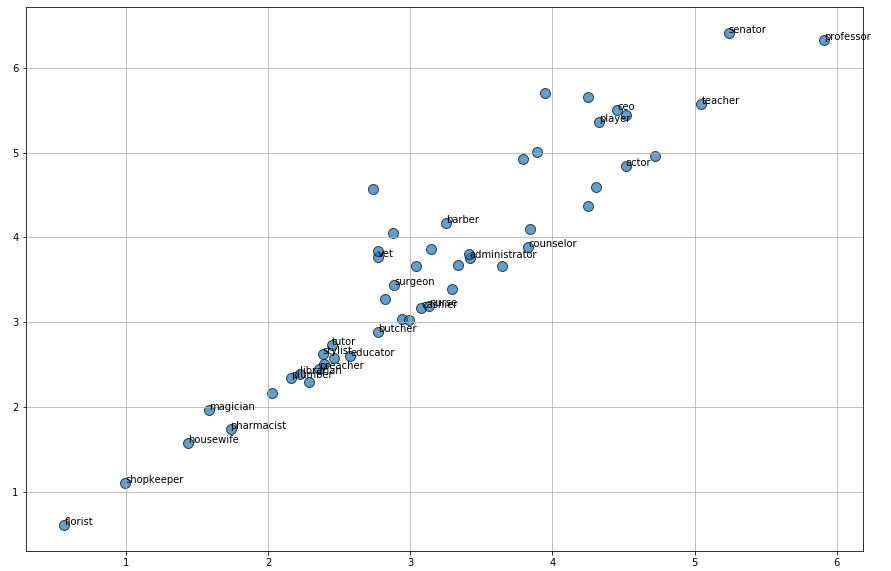
\includegraphics[width=25em]{biased_profession.png}}
			\caption{Result of clustering on male and female biased words}
			\label{profession-cluster-fig}
		\end{figure}
	\end{frame}
	
	\begin{frame}{Clustering on Common Words}
		\vspace{3mm}
		\begin{figure}[H]
			\centerline{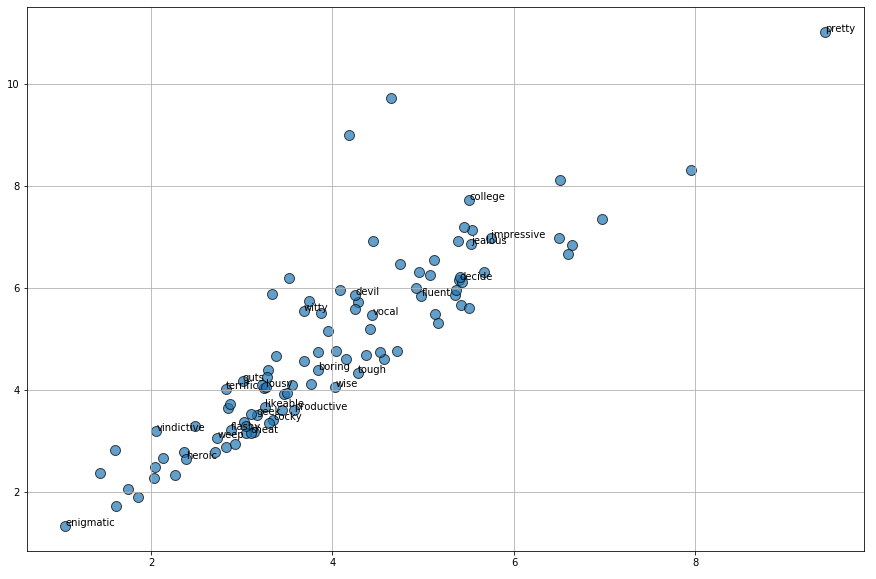
\includegraphics[width=25em]{biased_misc.png}}
			\caption{Result of clustering on male and female biased words}
			\label{common-cluster-fig}
		\end{figure}
	\end{frame}

	\section{Debiasing Word Embeddings}
		\begin{frame}{Debiasing using neutralisation of hard-debiasing}		
			Debiasing Professions based on Gender -- descending order \\
			('magician', 0.11574504) $\Rightarrow$ ('magician', 0.025625029836058758)
\\
			('carpenter', 0.046477906) $\Rightarrow$ ('carpenter', 0.0213426987806078) \\
			('gamer', 0.027397364) $\Rightarrow$ ('gamer', 0.0047532092934476355)
\\
			('soldier', 0.018920997) $\Rightarrow$ ('soldier', -0.0024024025014908745)
\\
			('servant', 0.009307076) $\Rightarrow$ ('servant', -0.0011262382124894582)
\\
			('barber', 0.0073357197) $\Rightarrow$ ('barber', 0.00432715694605746)
\\
			('engineer', -0.0022402948) $\Rightarrow$ ('engineer', -0.010558215937537)
\\
			('programmer', -0.016492) $\Rightarrow$ ('programmer', -0.0184568722608)
		\end{frame}
		\begin{frame}{Clustering on Profession after Debiasing}
			\vspace{3mm}
			\begin{figure}[H]
				\centerline{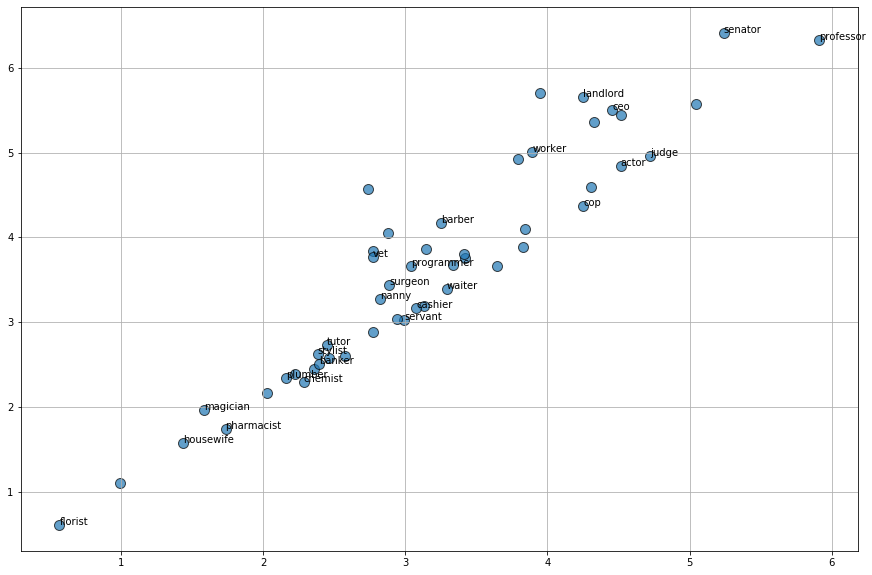
\includegraphics[width=25em]{dwe1.png}}
				\caption{Result of clustering on male and female biased words}
				\label{profession-debias-fig}
			\end{figure}
		\end{frame}
			
		\begin{frame}
			Debiasing Professions based on Race  -- descending order \\
		('servant', -0.014473432) $\Rightarrow$ ('servant', -0.01782729110568683)
		\\	
		('lawyer', -0.014795305) $\Rightarrow$ ('lawyer', -0.019276932830898832)
		\\
		('banker', -0.024144737) $\Rightarrow$ ('banker', -0.03891313915416421)
		\\
		('engineer', -0.039301794) $\Rightarrow$ ('engineer', -0.06321906512113795)
		\\
		('programmer', -0.06562963) $\Rightarrow$ ('programmer', -0.117997700482)
		\\
		('senator', -0.06934556) $\Rightarrow$ ('senator', -0.12828888982156872)
		\\
		('business', -0.08860369) $\Rightarrow$ ('business', -0.15978598382964143)
		\\	
		('scientist', -0.09481263) $\Rightarrow$ ('scientist', -0.16940044153193437)
		\\
		('worker', -0.11409591) $\Rightarrow$ ('worker', -0.19914736635361133)
		\\
		('ceo', -0.11503146) $\Rightarrow$ ('ceo', -0.1961109605431922)
		\\
		\end{frame}
		\begin{frame}{Clustering on Profession after Debiasing}
			\vspace{3mm}
			\begin{figure}[H]
				\centerline{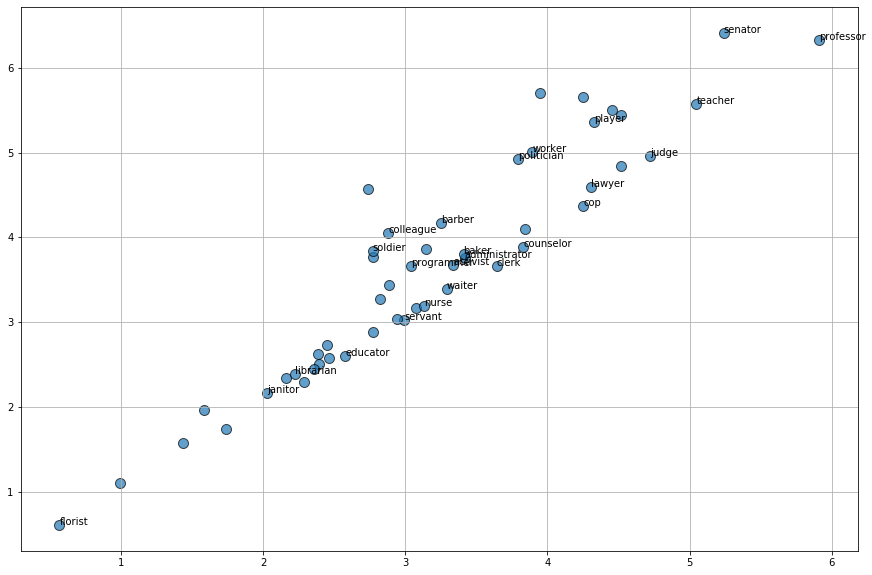
\includegraphics[width=25em]{dwe2.png}}
				\caption{Result of clustering on race biased words}
				\label{profession-debias-fig}
			\end{figure}
		\end{frame}
		\begin{frame}
			Debiasing Professions based on Religion  -- descending order \\
			('butcher', -0.0053771744) $\Rightarrow$ ('butcher', -0.005928319604247454)
			\\	
			('landlord', -0.008169426) $\Rightarrow$ ('landlord', -0.013176119539724127)
			\\
			('nurse', -0.010036137) $\Rightarrow$ ('nurse', -0.014683282999863613)
			\\
			('nanny', -0.011244472) $\Rightarrow$ ('nanny', -0.0167685528948944)
			\\
			('programmer', -0.06562963) $\Rightarrow$ ('programmer', -0.117997700482)
			\\
			('pharmacist', -0.015825728) $\Rightarrow$ ('pharmacist', -0.0209037176323)
			\\
			('clerk', -0.018447457) $\Rightarrow$ ('clerk', -0.0534647674024996)
			\\	
			('scientist', -0.09481263) $\Rightarrow$ ('scientist', -0.16940044153193437)
			\\
			('business', -0.027096914) $\Rightarrow$ ('business', -0.06418482800605033)
			\\
			('player', -0.034285568) $\Rightarrow$ ('player', -0.0754654672619229)
			\\
		\end{frame}
	\begin{frame}{Clustering on Profession after Debiasing}
		\vspace{3mm}
		\begin{figure}[H]
			\centerline{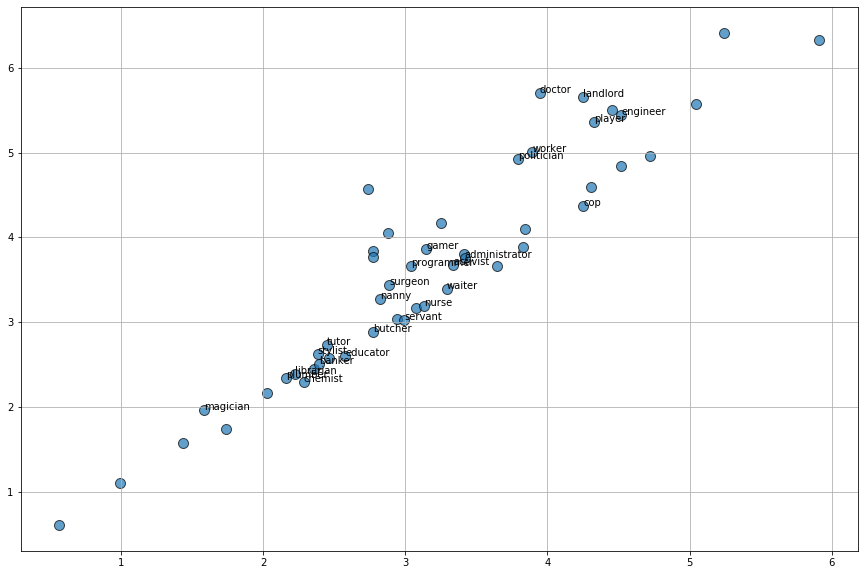
\includegraphics[width=25em]{dwe3.png}}
			\caption{Result of clustering on religion biased words}
			\label{profession-debias-fig}
		\end{figure}
	\end{frame}
	
	\begin{frame}
		Debiasing Misc. Words based on Gender  -- descending order \\
		('swear', 0.21706519) $\Rightarrow$ ('swear', 0.04715369477049303)
		\\	
		('filthy', 0.20151068) $\Rightarrow$ ('filthy', 0.026021153148268236)
		\\
		Debiasing Misc. Words based on Race  -- descending order \\
		('comical', -0.0012468412) $\Rightarrow$ ('comical', -0.007484548413770923)
		\\	
		('maths', -0.015644163) $\Rightarrow$ ('maths', -0.027991168738123316)
		\\
		Debiasing Misc. Words based on Religion  -- descending order \\
		('guts', 0.0026711777) $\Rightarrow$ ('guts', 0.0017492761220381202)
		\\	
		('backpack', -0.0016981252) $\Rightarrow$ ('backpack', -0.01208588318522)
	\end{frame}
	\begin{frame}{Clustering on Profession after Debiasing}
		\vspace{3mm}
		\begin{figure}[H]
			\centerline{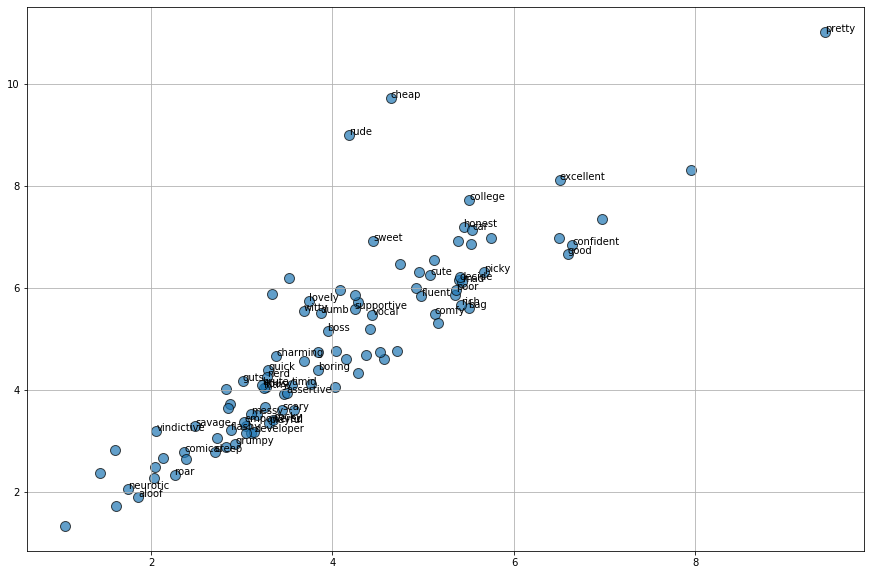
\includegraphics[width=25em]{dwe4.png}}
			\caption{Result of clustering on gender biased words}
			\label{profession-debias-fig}
		\end{figure}
	\end{frame}
\begin{frame}{Clustering on Profession after Debiasing}
	\vspace{3mm}
	\begin{figure}[H]
		\centerline{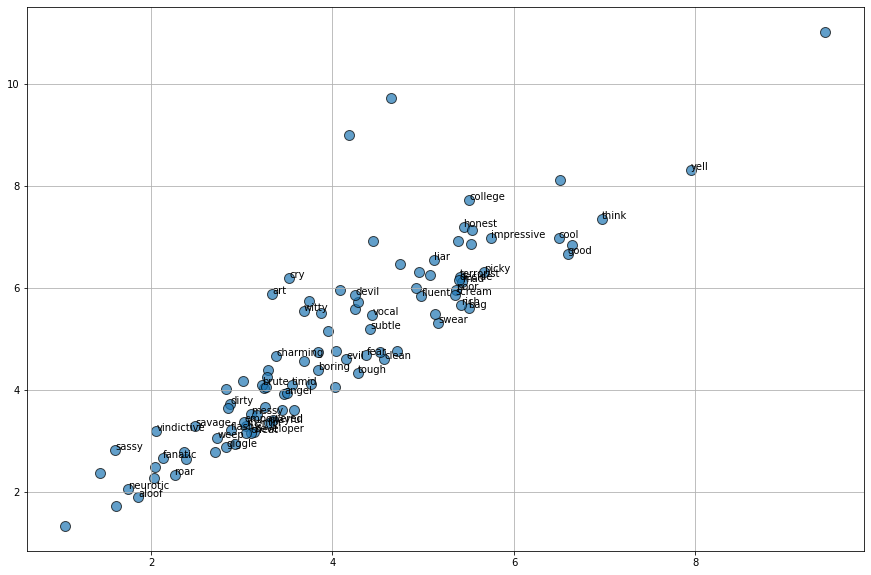
\includegraphics[width=25em]{dwe5.png}}
		\caption{Result of clustering on race biased words}
		\label{profession-debias-fig}
	\end{figure}
\end{frame}
\begin{frame}{Clustering on Profession after Debiasing}
	\vspace{3mm}
	\begin{figure}[H]
		\centerline{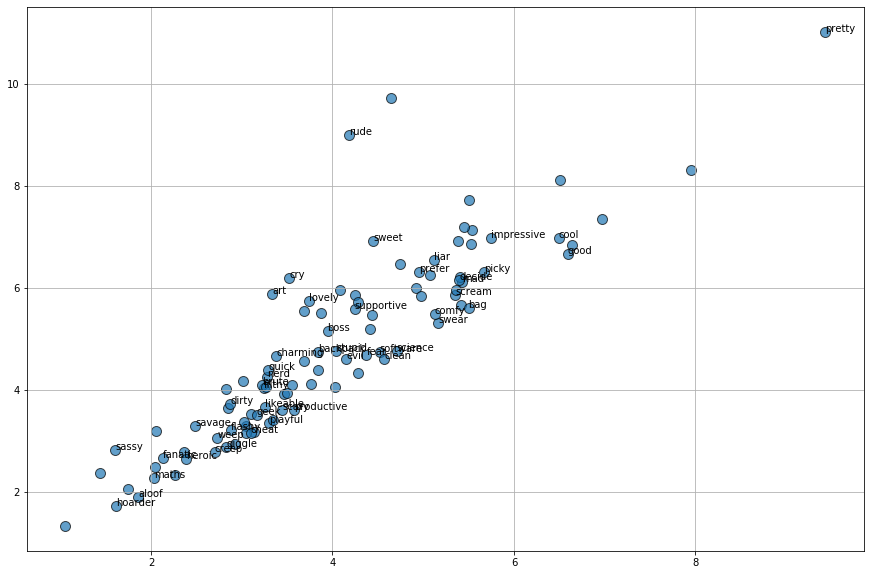
\includegraphics[width=25em]{dwe6.png}}
		\caption{Result of clustering on religion biased words}
		\label{profession-debias-fig}
	\end{figure}
\end{frame}
		
	
	

	\section{Proposed Algorithm}
		\begin{frame}{Proposed algorithm}
			\begin{itemize}
				\item Pre-processing dataset --> add sentences by inverting the gender, races, religion, etc. --> appending them to create a new dataset.
				\item Debiasing during pre-processing as with (Zhao et al.)
				\item  Analyse `biased' words --> projecting them to biased sub-space and debias (Bolukbasi et al.)
				\item After identifying these words --> correlated with each other --> distances between the words clustering together should also be equalised.
			\end{itemize}
		\end{frame}
	
		
	\section{Conclusion}
	\begin{frame}{Conclusion}
		\begin{itemize}
			\item Project involved exploring various biases in word embeddings
			\item Word embeddings trained on the Reddit dataset were explored
			\item Attempt to debias using the traditional hard-debiasing method was done
			\item Debiasing happened on a superficial level
			\item Approach proposed that may address the issue
		\end{itemize}
	\end{frame}

	\section{Future Scope}
	\begin{frame}{Future Scope}
		\begin{itemize}
			\item Implement proposed algorithm
			\item Empirically test performance of proposed model
			\item Explore how biases are encoded in word embeddings
		\end{itemize}
	\end{frame}
	
	
	\section{References}
	\begin{frame}[allowframebreaks]{References}
		\small{
				\begin{thebibliography}{10}
				
				\bibitem{1} Hila Gonen, Yoav Goldberg, \textit{Lipstick on a Pig: Debiasing methods cover up systematic gender biases in word embeddings but do not remove them}, \url{https://arxiv.org/pdf/1903.03862.pdf}
				\bibitem{2} Tolga Bolukbasi, et al., \textit{Man is to Computer Programmer as Woman is to Homemaker? Debiasing Word Embeddings}, \url{https://arxiv.org/pdf/1607.06520.pdf}
				\bibitem{3} Jieyu Zhao, et al., \textit{Learning Gender-Neutral Word Embeddings}, \url{https://arxiv.org/pdf/1809.01496.pdf}
				\bibitem{4} Sevtap Duman, et al., \textit{(Visualization of) gender bias in word embeddings}, \url{http://wordbias.umiacs.umd.edu/}
				\bibitem{5}Aylin Caliskan, et al., \textit{Semantics derived automatically from language corpora contain human-like biases}, \url{https://arxiv.org/pdf/1608.07187.pdf}
				\bibitem{6}Nikhil Garg, et al., \textit{Word embeddings quantify 100 years of gender and ethnic stereotypes}, \url{https://arxiv.org/pdf/1711.08412.pdf}
				\bibitem{7} Thomas Manzini, et al., \textit{Black is to Criminal as Caucasian is to Police:Detecting and Removing Multiclass Bias in Word Embeddings}, \url{https://arxiv.org/pdf/1904.04047v1.pdf}
				\bibitem{8} Harini Suresh, John V. Guttag, \textit{A Framework for Understanding Unintended Consequences of Machine Learning}, \url{https://arxiv.org/pdf/1901.10002.pdf}
				\bibitem{9} Alex Fefegha, \textit{Racial Bias and Gender Bias Examples in AI systems}, \url{https://peopleofcolorintech.com/articles/racial-bias-and-gender-bias-examples-in-ai-systems/}
				\bibitem{10}Marianne Bertrand, Sendhil Mullainathan, \textit{Are Emily and Greg More Employable than Lakisha and Jamal? A Field Experiment on LaborMarket Discrimination}, \url{https://www2.econ.iastate.edu/classes/econ321/Orazem/bertrand_emily.pdf}
				\bibitem{11} Thomas Manzini, et al., \textit{Debiasing Multiclass Word Embeddings}, \url{https://github.com/TManzini/DebiasMulticlassWordEmbedding}
				\bibitem{12}Ella Rabinovich, Shuly Wintner, \textit{The Reddit-L2 corpus}, \url{http://cl.haifa.ac.il/projects/L2/}
				
			\end{thebibliography}
		}
		
	\end{frame}
	
\end{document}
